\documentclass[a4paper,8pt]{article}
\pagestyle{plain}


\usepackage[utf8]{inputenc}
\usepackage{fancyhdr}
\usepackage[margin=2cm,foot=1cm]{geometry}
\usepackage[T1]{fontenc}
\usepackage{hyperref}
\usepackage{ragged2e}
\usepackage{pgf-umlcd}
\usepackage{graphicx,multicol}

\hypersetup{
	colorlinks,
	linkcolor={blue!80!black},
	citecolor={green!80!black},
	urlcolor={red!80!black}
}


% Used to set numbering of the content
\setcounter{tocdepth}{2}
\setcounter{secnumdepth}{3}

%%
% Math packages
\usepackage[utf8]{inputenc}
\usepackage{mathtools}
\usepackage{amssymb}
\usepackage{bm}
\usepackage{amsthm}
\usepackage{bbm}
\usepackage{amsmath}
\usepackage{rotating}
\usepackage{mathrsfs}
\usepackage{tikz-cd}
\usepackage{float}
\usepackage{enumitem}

\graphicspath{ {./images/} }

%%
% Math Commands
\def\upint{\mathchoice%
	{\mkern13mu\overline{\vphantom{\intop}\mkern7mu}\mkern-20mu}%
	{\mkern7mu\overline{\vphantom{\intop}\mkern7mu}\mkern-14mu}%
	{\mkern7mu\overline{\vphantom{\intop}\mkern7mu}\mkern-14mu}%
	{\mkern7mu\overline{\vphantom{\intop}\mkern7mu}\mkern-14mu}%
	\int}
\def\lowint{\mkern3mu\underline{\vphantom{\intop}\mkern7mu}\mkern-10mu\int}
\usepackage{tikz}
\newcommand{\N}{\mathbb{N}}
\newcommand{\Lagr}{\mathcal{L}}
\newcommand{\R}{\mathbb{R}}
\newcommand{\Q}{\mathbb{Q}}
\newcommand{\C}{\mathbb{C}}
\newcommand{\x}{\mathbf{x}}
\newcommand{\F}{\mathbf{F}}
\newcommand{\f}{\mathbf{f}}
\newcommand{\y}{\mathbf{y}}
\renewcommand{\b}{\mathbf{b}}
\renewcommand{\c}{\mathbf{c}}
\renewcommand{\a}{\mathbf{a}}
\newcommand{\h}{\mathbf{h}}
\newcommand{\g}{\mathbf{g}}
\newcommand{\z}{\mathbf{z}}
\newcommand{\ze}{\mathbf{0}}
\newcommand{\Z}{\mathbb{Z}}
\newcommand{\norm}[1]{\left\lVert#1\right\rVert}
\newcommand{\abs}[1]{\left\lvert#1\right\rvert}
\newcommand{\brk}[1]{ \left[#1\right] }
\newcommand{\brc}[1]{ \left\{#1\right\} }
\newcommand{\paren}[1]{ \left(#1\right) }
\newcommand{\normop}[1]{\left\lVert#1\right\rVert_\text{op}}
\newcommand{\LL}{\mathcal{L}}
\newcommand{\uni}{\overset{\text{uni}}{\to}}
\DeclareMathOperator{\diam}{diam}
\newcommand{\Prr}[1]{\text{Pr}\left(#1\right)}
\newcommand{\code}[1]{\texttt{#1}}

\definecolor{dartmouthgreen}{rgb}{0.05, 0.5, 0.06}
\definecolor{egyptianblue}{rgb}{0.06, 0.2, 0.65}
\definecolor{dukeblue}{rgb}{0.0, 0.0, 0.61}
\definecolor{jazzberryjam}{rgb}{0.65, 0.04, 0.37}
\definecolor{magenta}{HTML}{EC008C}

%%
% Self-defined useful shortcuts
\newcommand{\isomorp}{\xrightarrow{\sim}}
\newcommand{\hlt}[1]{\textit{{\color{dukeblue}#1}}}
\newcommand{\impt}[1]{\textit{{\color{jazzberryjam}#1}}}
\newcommand{\qntype}[1]{\textit{{\color{dartmouthgreen}#1}}}
\newcommand{\soln}[1]{\textit{{\color{magenta}#1}}}
\newcommand{\gcds}[1]{\textnormal{gcd}#1}
\newcommand{\mins}[1]{\textnormal{min}#1}
\newcommand{\maxs}[1]{\textnormal{max}#1}
\newcommand{\lcms}[1]{\textnormal{lcm}#1}
\newcommand{\degs}[1]{\textnormal{deg}#1}
\newcommand{\exps}[1]{\textnormal{exp}#1}
\newcommand{\tors}[1]{\textnormal{Tor}#1}
\newcommand{\homs}[1]{\textnormal{Hom}#1}
\newcommand{\anns}[1]{\textnormal{Ann}#1}

%%
\setcounter{section}{0}
% Set up math tools
\theoremstyle{theorem}
\newtheorem{theorem}{Theorem}[section]
\newtheorem{corollary}[theorem]{Corollary}
\newtheorem{lemma}[theorem]{Lemma}
\newtheorem{proposition}[theorem]{Proposition}
\newtheorem{qnbank}[theorem]{Question Bank}
\let\oldqnbank\qnbank
\renewcommand{\qnbank}{\oldqnbank\normalfont}
\newtheorem{algorithm}[theorem]{Algorithm}
\let\oldalgorithm\algorithm
\renewcommand{\algorithm}{\oldalgorithm\normalfont}
\newtheorem{definition}[theorem]{Definition}
\let\olddefinition\definition
\renewcommand{\definition}{\olddefinition\normalfont}
\newtheorem{example}[theorem]{Example}
\let\oldexample\example
\renewcommand{\example}{\oldexample\normalfont}
\newtheorem{remark}[theorem]{Remark}
\let\oldremark\remark
\renewcommand{\remark}{\oldremark\normalfont}


\title{MA5251 Project 2}
\author{Li Xuanguang, A0154735B}

\begin{document}
\maketitle

\section{Numerical Method Discussion}

\noindent
We are given the burgers equation
\begin{align} 
\frac{\partial u}{\partial t}& + \frac{\partial}{\partial x}\left(\frac{u^{2}}{2}\right) = 0.02 \frac{\partial^2 u}{\partial x^2} \nonumber \\
u&(-1,t)=1, u(1, t) = -1 \nonumber \\
u(x,0) &= u_0 (x) = -\sin \left(\frac{5}{2} \pi x \right) \nonumber
\end{align}

\noindent
First, we take the approximation 
\begin{equation}
u_N(x,t) = \sum\limits_{k=0}^{N} \hat{u}_k(t) T_k(x) \nonumber
\end{equation}

\noindent
As there is a nonlinear term in the equation, choose the right collocation points first and use interpolation to approximate the result. We use Gauss-Lobatto notes:
\begin{equation}
x_j = \cos \left(\frac{j \pi}{n}\right), \ \ j = 0, 1, \ldots, n \nonumber
\end{equation}

\noindent
After approximating the nonlinear term $\frac{u^2}{2}$, we deal with the approximation after taking derivative with respect to $x$. By lecture 19, we have the following recursion for approximation:
\begin{equation}
u'_N(x) = \sum\limits_{k=0}^{N} \hat{u}_k^{(1)}T_k(x) \nonumber
\end{equation}
where $u^{(1)}_N = 0$, $u^{(1)}_{N-1} = 2N \hat{u}_N$, $\hat{u}^{(1)}_{k-1} = \frac{\hat{u}^{(1)}_{k+1} + 2k \hat{u}_k}{c_{k-1}}$.\\
For the term $0.02 \frac{\partial^2 u}{\partial x^2}$, the differentiation is done twice.\\

\noindent
Next, we use semi-discretisation with the following:
\begin{equation}
\frac{\partial u_N}{\partial t} (x_j, t) = \frac{\partial f_N}{\partial x} (x_j, t), \ \ j = 1, \ldots, N-1 \nonumber
\end{equation}
where
\begin{equation}
f_N = I_N \left(- \frac{u^2_N}{2} \right) + 0.02 \frac{\partial u_N}{\partial x} \nonumber
\end{equation}
and
\begin{align}
u_N(-1,t) &= 1 \nonumber \\
u_N(1,t) &= -1 \nonumber \\
u_N(x,0) &= I_N u_0(x) \nonumber \\
u_0(x) &= -\sin \left(\frac{5}{2} \pi x \right) \nonumber
\end{align}

We then apply the third-order RK method to get the results.

\section{Numerical Results and Discussion}

The code is written in Python, adapted off Prof Cai Zhenning's Matlab code in Lecture 19.\\

\noindent
We run the code with the following parameters:
\begin{enumerate}[label=\arabic*.]
\setlength{\itemsep}{0pt}
\item \code{N = 32}
\item \code{T = 5}
\item \code{$\triangle$t = 0.001}
\item \code{$\triangle$tp = 0.3} (timestep for print, used to print outputs)
\end{enumerate}

As seen from the figures (next page), the curve reaches steady state by $t=3.3$.

\begin{figure}[h!]
\begin{multicols}{2}
\centering
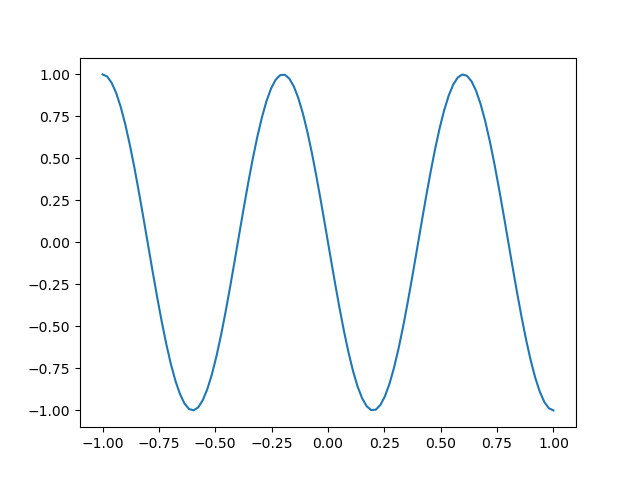
\includegraphics[width=1\linewidth]{t0.0_plot.png}\\
State at $t=0.0$
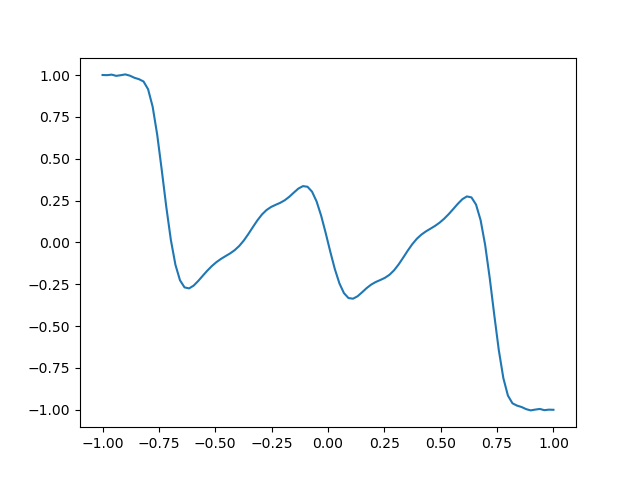
\includegraphics[width=1\linewidth]{t0.6_plot.png}\\
State at $t=0.6$
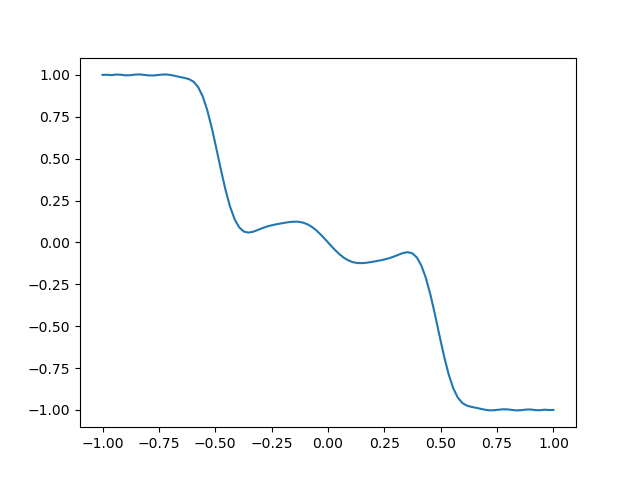
\includegraphics[width=1\linewidth]{t1.2_plot.png}\\
State at $t=1.2$
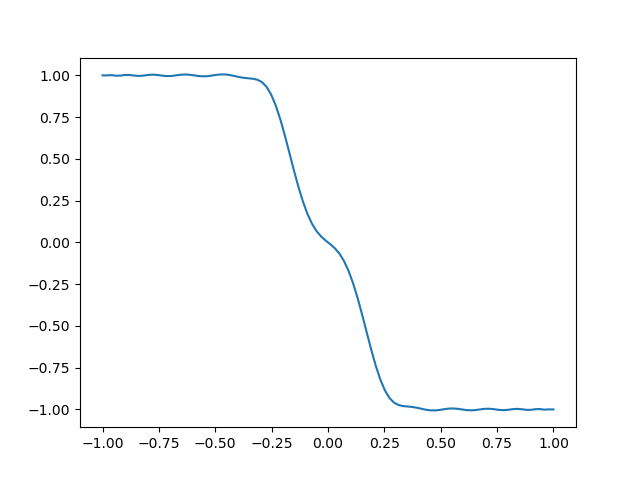
\includegraphics[width=1\linewidth]{t1.8_plot.png}\\
State at $t=1.8$
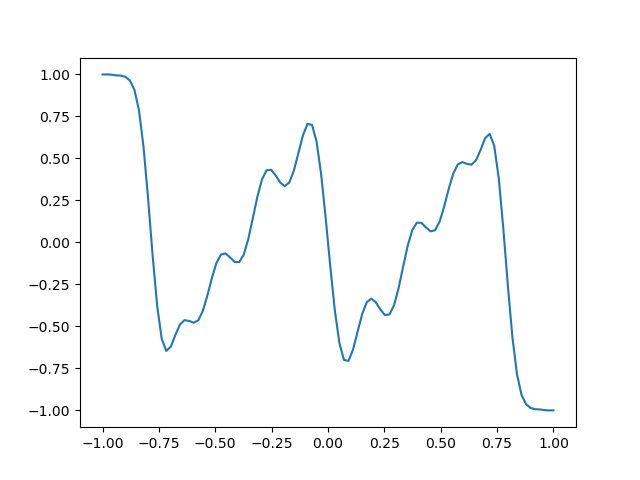
\includegraphics[width=1\linewidth]{t0.3_plot.png}\\
State at $t=0.3$
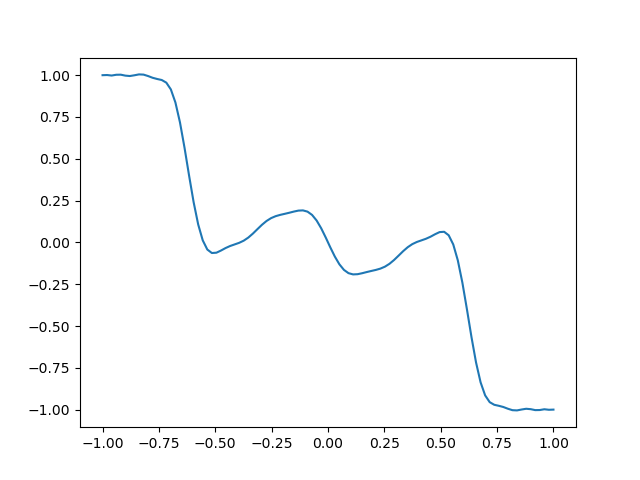
\includegraphics[width=1\linewidth]{t0.9_plot.png}\\
State at $t=0.9$
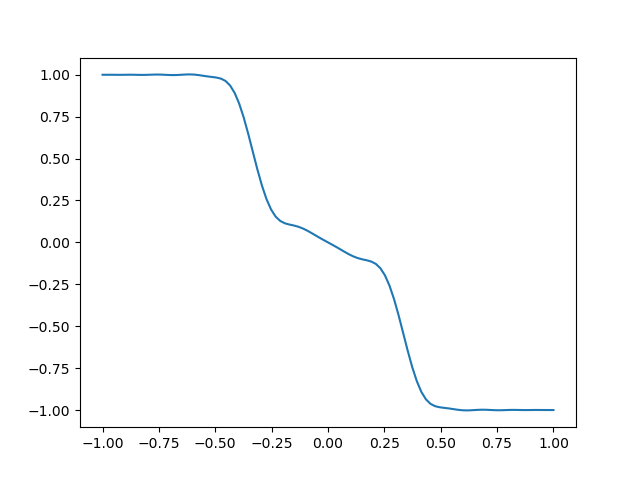
\includegraphics[width=1\linewidth]{t1.5_plot.png}\\
State at $t=1.5$
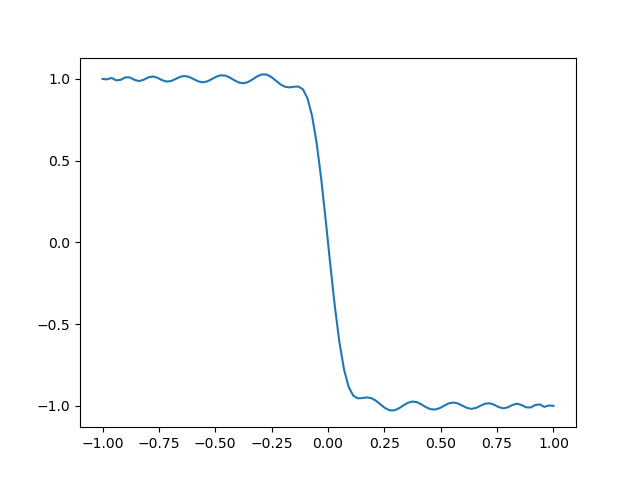
\includegraphics[width=1\linewidth]{t2.1_plot.png}\\
State at $t=2.1$
\end{multicols}
\end{figure}

\newpage

\begin{figure}[h!]
\begin{multicols}{2}
\centering
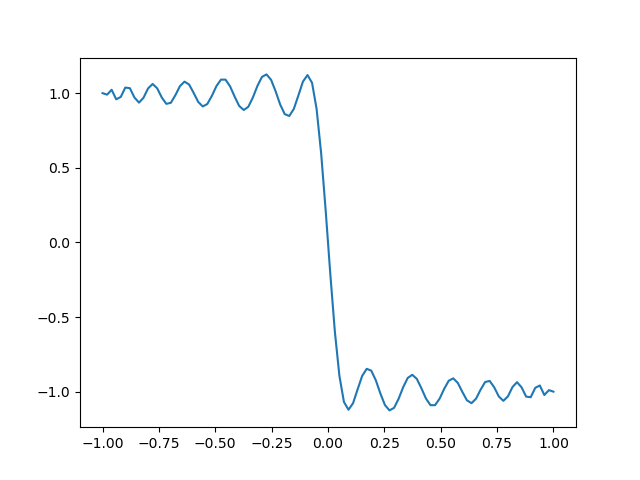
\includegraphics[width=1\linewidth]{t2.4_plot.png}\\
State at $t=2.4$
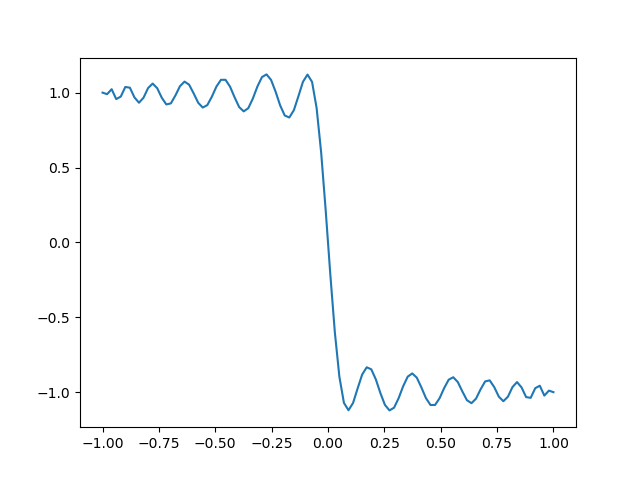
\includegraphics[width=1\linewidth]{t3.0_plot.png}\\
State at $t=3.0$
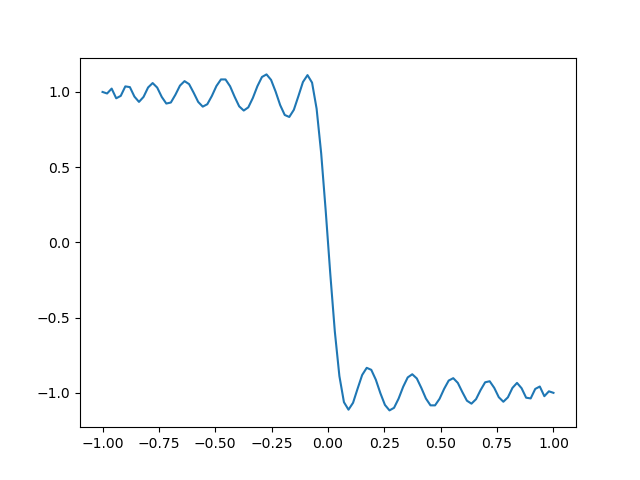
\includegraphics[width=1\linewidth]{t3.6_plot.png}\\
State at $t=3.6$
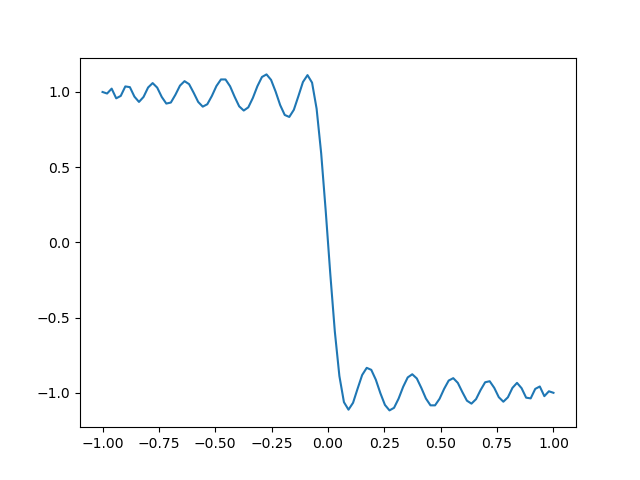
\includegraphics[width=1\linewidth]{t4.2_plot.png}\\
State at $t=4.2$
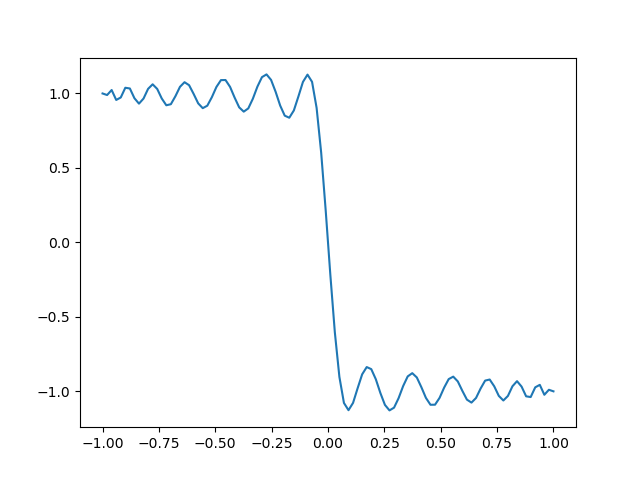
\includegraphics[width=1\linewidth]{t2.7_plot.png}\\
State at $t=2.7$
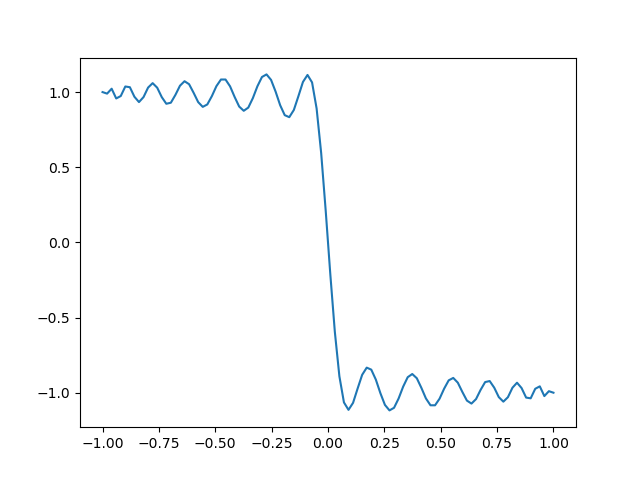
\includegraphics[width=1\linewidth]{t3.3_plot.png}\\
State at $t=3.3$
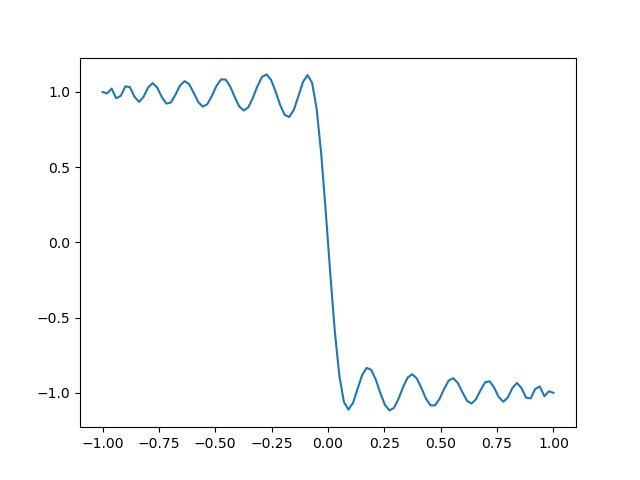
\includegraphics[width=1\linewidth]{t3.9_plot.png}\\
State at $t=3.9$
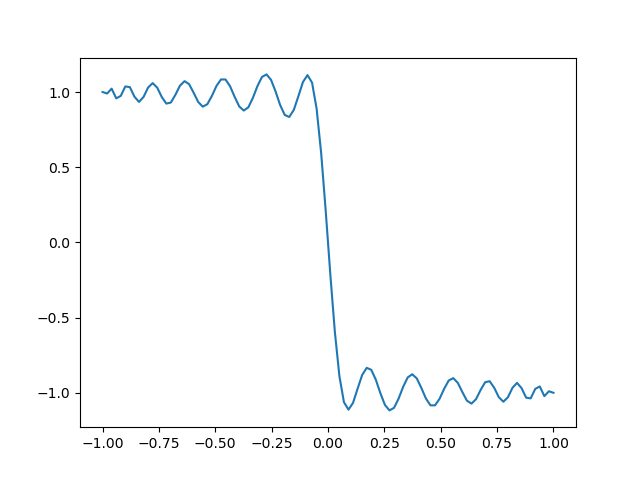
\includegraphics[width=1\linewidth]{t4.5_plot.png}\\
State at $t=4.5$
\end{multicols}
\end{figure}

\end{document}
